\documentclass[11pt,oneside]{book}
\usepackage[margin=1.2in]{geometry}
\usepackage[toc,page]{appendix}
\usepackage{graphicx}
\usepackage{natbib}
\usepackage{lipsum}
\usepackage{caption}
\usepackage[T1]{fontenc}
\usepackage{titlesec, blindtext, color}
\usepackage{xcolor,tikz}
\usepackage{tikz-cd}
\usepackage{caption}
\usepackage{subcaption}
\usetikzlibrary{patterns}
\usetikzlibrary{decorations.markings}
\usetikzlibrary{decorations.pathmorphing}
% \usepackage{amsmath,amssymb,amsthm,mathrsfs,amsfonts,xfrac,pifont,bbold,physics}
\usepackage[utf8]{inputenc}
\usepackage{amsthm}
\usepackage{pgfplots}
\usepackage[breakable, theorems, skins]{tcolorbox}
\usepackage[colorlinks = true,
            linkcolor = red,
            urlcolor  = blue,
            citecolor = red,
            anchorcolor = red]{hyperref}
\usepackage{enumitem}
\usepackage{TemplateMatma}
\usepackage{TemplateNotatkiPE}

\tikzset{
    partial ellipse/.style args={#1:#2:#3}{
        insert path={+ (#1:#3) arc (#1:#2:#3)}
    }
}


\renewcommand{\vec}[1]{\underline{#1}}

% -------------------------------------------------------------------
% Theorem Styles
% -------------------------------------------------------------------

\theoremstyle{definition} % Define theorem styles here based on the definition style (used for definitions and examples)
\newtheorem*{definition}{Definition}

\theoremstyle{plain} % Define theorem styles here based on the plain style (used for theorems, lemmas, propositions)
\newtheorem{theorem}{Theorem}[section]
\newtheorem{axiom}{Axiom}
\newtheorem{corollary}[theorem]{Corollary}
\newtheorem{lemma}[theorem]{Lemma}
\newtheorem{proposition}[theorem]{Proposition}
\newtheorem{postulate}{Postulate}

\theoremstyle{remark} % Define theorem styles here based on the remark style (used for remarks and notes)
\newtheorem*{solution}{Solution}


\newtheoremstyle{underline}% name
{}        % Space above, empty = `usual value'
{}              % Space below
{}              % Body font
{}    % Indent amount (empty = no indent, \parindent = para indent)
{}              % Thm head font
{.}             % Punctuation after thm head
{1.5mm}         % Space after thm head: \newline = linebreak
{{\underline{\textit{\thmname{#1}\thmnumber{ #2}}~\thmnote{(#3)}\unskip}}}  % Thm head spec

\theoremstyle{underline}

\newtheorem{remark}[theorem]{Remark}
\newtheorem{example}[theorem]{Example}
\newtheorem{claim}[theorem]{Claim}
\newtheorem{exercise}[theorem]{Exercise}
\newtheorem*{terminology}{Terminology}
\newtheorem*{notation}{Notation}
\newtheorem*{convention}{Convention}



% -------------------------------------------------------------------
% Chapter Headings
% -------------------------------------------------------------------

\setcounter{chapter}{0}

\makeatletter
\renewcommand{\@chapapp}{Lecture}
\makeatother
\definecolor{lightergray}{rgb}{0.9,0.9,0.9}

\usepackage{titlesec}
\titleformat{\section}{\large\bfseries\raggedright}{}{0em}{\colorsection}[\titlerule]
\titleformat{name=\section,numberless}{\large\scshape\bfseries\raggedright}{}{0em}{\colorsectionnonumber}[\titlerule]

\titleformat{\subsection}{\bfseries\raggedright}{}{0em}{\colorsubsection}
\titleformat{name=\subsection,numberless}{\bfseries\raggedright}{}{0em}{\colorsubsectionnonumber}

\newcommand{\colorsection}[1]{%
    \colorbox{lightergray}{\parbox{\dimexpr\textwidth-2\fboxsep}{\thesection\ \ #1}}}
\newcommand{\colorsectionnonumber}[1]{%
    \colorbox{lightergray}{\parbox{\dimexpr\textwidth-2\fboxsep}{#1}}}
    
\newcommand{\colorsubsection}[1]{%
    \colorbox{lightergray}{\parbox{\dimexpr\textwidth-2\fboxsep}{\thesubsection\ #1}}}
\newcommand{\colorsubsectionnonumber}[1]{%
    \colorbox{lightergray}{\parbox{\dimexpr\textwidth-2\fboxsep}{#1}}}
    
\definecolor{gray75}{gray}{0.75}
\newcommand{\hsp}{\hspace{20pt}}
\titleformat{\chapter}[hang]{\Huge\bfseries}{\thechapter\hsp\textcolor{gray75}{|}\hsp}{0pt}{\Huge\bfseries}

\title{Hydrodynamics and elasticity,\\ Lecture notes}
\author{Mikołaj Duch}

\begin{document}

  \maketitle
  \frontmatter

  % -------------------------------------------------------------------
  % Contents
  % -------------------------------------------------------------------

  \tableofcontents

  % -------------------------------------------------------------------
  % Main sections 
  % -------------------------------------------------------------------

  \mainmatter

  \chapter{Basic definitions}


  \section{Organization}
  Course web page: \url{https://www.fuw.edu.pl/~mklis/hydro2022.html}
  

  Requirements to obtain credit:
  \begin{itemize}
    \item Homework ($30\%$),
    \item Midterm exam ($35\%$),
    \item Written exam ($35\%$),
    \item Oral exam (optional, only improves).
  \end{itemize}

  % Climate is a nice playground for hydrodynamics.

  \section{Basic laws}

  \begin{example}
    Out of context Navier-Stokes equations:
    \begin{displaymath}
      \ptf{\vec u}{t} + \vec u \cdot \nabla \vec u = - \frac{1}{\rho} \nabla p + \nu\nabla^2 \vec u,
    \end{displaymath}
    \begin{displaymath}
      \nabla \cdot \vec u = 0.
    \end{displaymath}
    where $\vec u(\vec r,t)$ is a fluid velocity vector field, $\rho(\vec r,t)$ is a fluid density, 
    $p(\vec r, t)$ is a pressure, $\nu$ is a kinematic viscosity.
  \end{example}

  \sep


  Continuum hypothesis states that
  \begin{displaymath}
    \rho = \frac{\delta\eta}{\delta \nu},
  \end{displaymath}
  where $\eta$ is a number of particles in a region and $\nu$ is a volume of this region.
  Of course if the volume $\nu$ is small enough $\rho$ is may vary a lot (obviously it may not even be continuous).
  There is however such volume $V$ which is ,,big enough'', so that for $\nu > V$ $\rho$ does not vary ,,that much''.


  \begin{figure}[h]
    \begin{center}
      \begin{subfigure}{0.3\linewidth}
        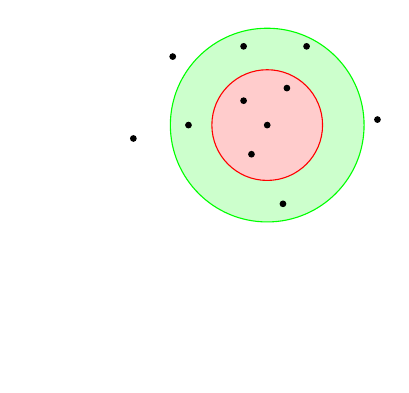
\begin{tikzpicture}
          \draw[white] (0,0) circle (1pt);
          \begin{scope}[shift={(3cm, 3cm)}]
            \draw[fill=green!20, draw=green] (0,0) circle (35pt);
            \filldraw[fill=red!20, draw=red] (0,0) circle (20pt);
            \filldraw[black] (0,0) circle (1pt);
            \filldraw[black] (0.5,1) circle (1pt);
            \filldraw[black] (-0.3,1) circle (1pt);
            \filldraw[black] (0.2,-1) circle (1pt);
            \filldraw[black] (-1,0) circle (1pt);
            \filldraw[black] (-0.3,0.31) circle (1pt);
            \filldraw[black] (0.25,0.47) circle (1pt);
            \filldraw[black] (-0.20,-0.37) circle (1pt);
            \filldraw[black] (-1.7,-0.17) circle (1pt);
            \filldraw[black] (-1.2,0.87) circle (1pt);
            \filldraw[black] (1.4,0.07) circle (1pt);
          \end{scope}
        \end{tikzpicture}
      \end{subfigure}%
      \begin{subfigure}{0.7\linewidth}
        \centering
        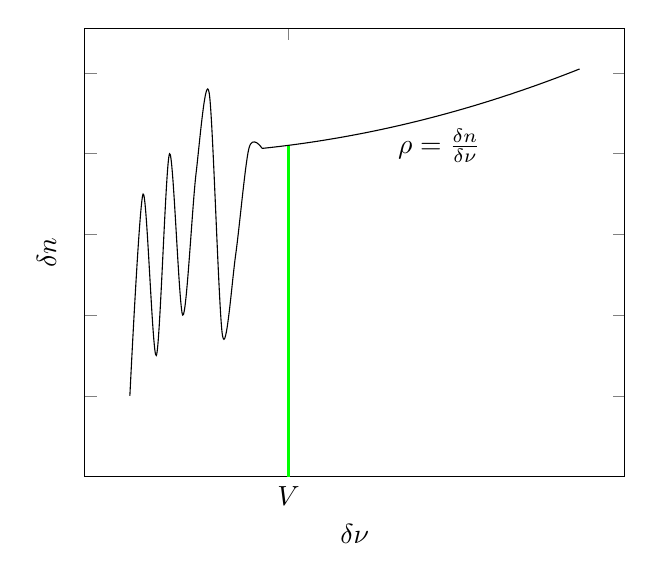
\begin{tikzpicture}
          \begin{axis}[
              xtick = {13},
              xticklabels = {$V$},
              yticklabels = {},
              ymin=0,
              xlabel = {$\delta \nu$},
              ylabel = {$\delta n$}
            ]
            \addplot[smooth] coordinates {
              (1, 2)
              (2, 7)
              (3, 3)
              (4, 8)
              (5, 4)
              (6, 7.5)
              (7, 9.5)
              (8, 3.5)
              (9, 5.5)
              (10, 8.132)
              (11, 8.132)
              % (12.5, 8.1)
              % (15, 8.3)
              % (17.5, 8.5)
              % (20, 9)
              % (30, 9.5)
            };
            \addplot [
              domain = 11:35,
              samples = 100
            ]
            {0.01 * (0.2 * x^2 - x + 800)};
            \addplot +[mark=none, color=green, thick] coordinates {(13, -1) (13, 8.2)};

          \end{axis}
            \node at (4.5, 4.2) {$\rho = \frac{\delta n}{\delta \nu}$};
        \end{tikzpicture}
      \end{subfigure}

    \end{center}
    \label{fig:0}
  \end{figure}


  Since matter is not continuous, we can't speak of a density at a point (in a mathematical sense) and
  thus, when we use the phrase ,,point'' we mean ,,at a point for homogeneous physical system''.

  We also introduce length scale separation % for 

  \begin{displaymath}
    \begin{matrix}
      \tm{molecular length scale} & \ll & \nu^{\frac{1}{3}} & \ll & L.
    \end{matrix}
  \end{displaymath}
  We call those characteristic length scales ,,\emph{micro}'', ,,\emph{muso}'' and ,,\emph{macro}'' respectively.
  

  \subsection{Equilibrium thermodynamics}
  \begin{figure}[H]
    \begin{subfigure}{0.5\linewidth}
      \centering
      \begin{tikzpicture}
        \node[anchor = south west] (image) at (0,0)
        {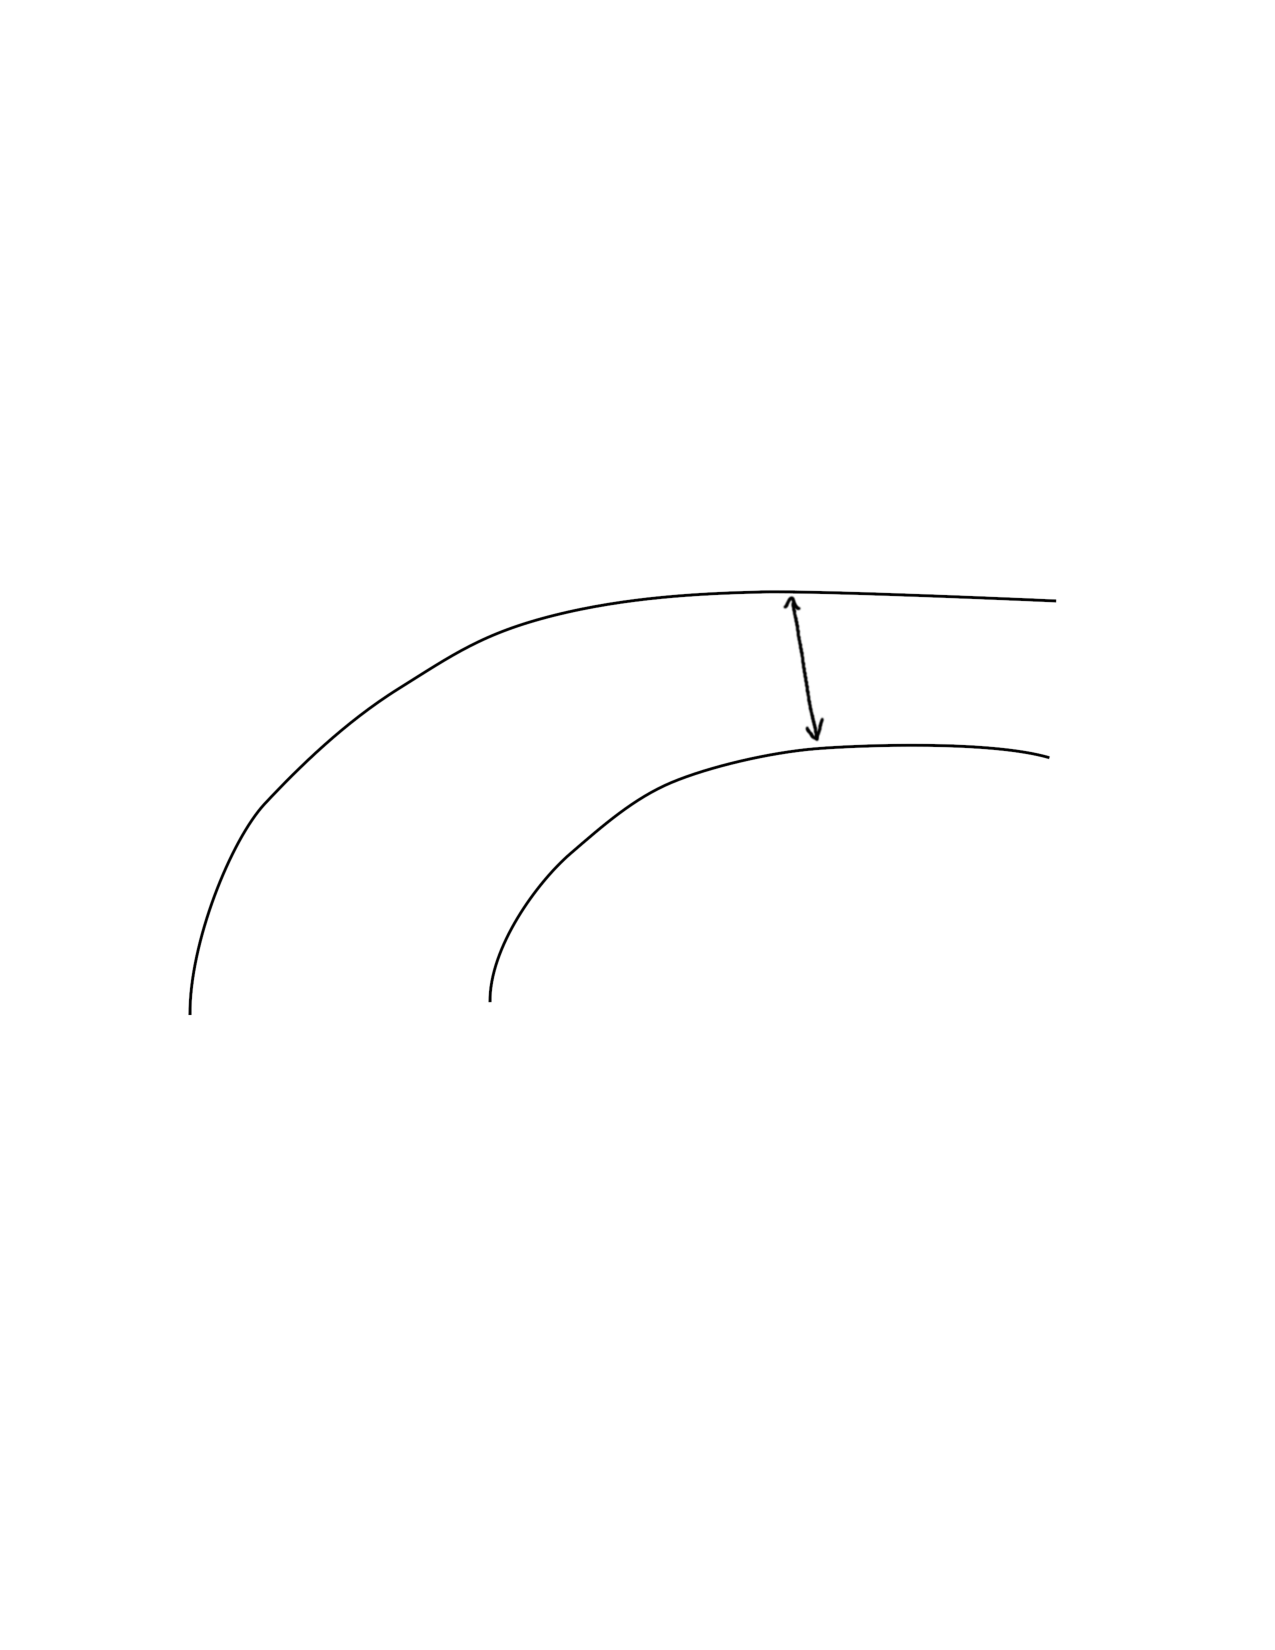
\includegraphics[width=\textwidth]{./images/00river.pdf}};
        \begin{scope}[x={(image.south east)}, y={(image.north west)}]
          \node at (0.35, 0.5) {$\vec u(\vec r, t)$};
          \node at (0.65, 0.5) {river};
          \draw [-stealth] (0.4,0.52) -- (0.5,.58);
        \end{scope}
      \end{tikzpicture}

    \end{subfigure}
    \begin{subfigure}{0.5\linewidth}
      \centering
      \begin{tikzpicture}
        \node[anchor=south west] (image) at (0,0)
        {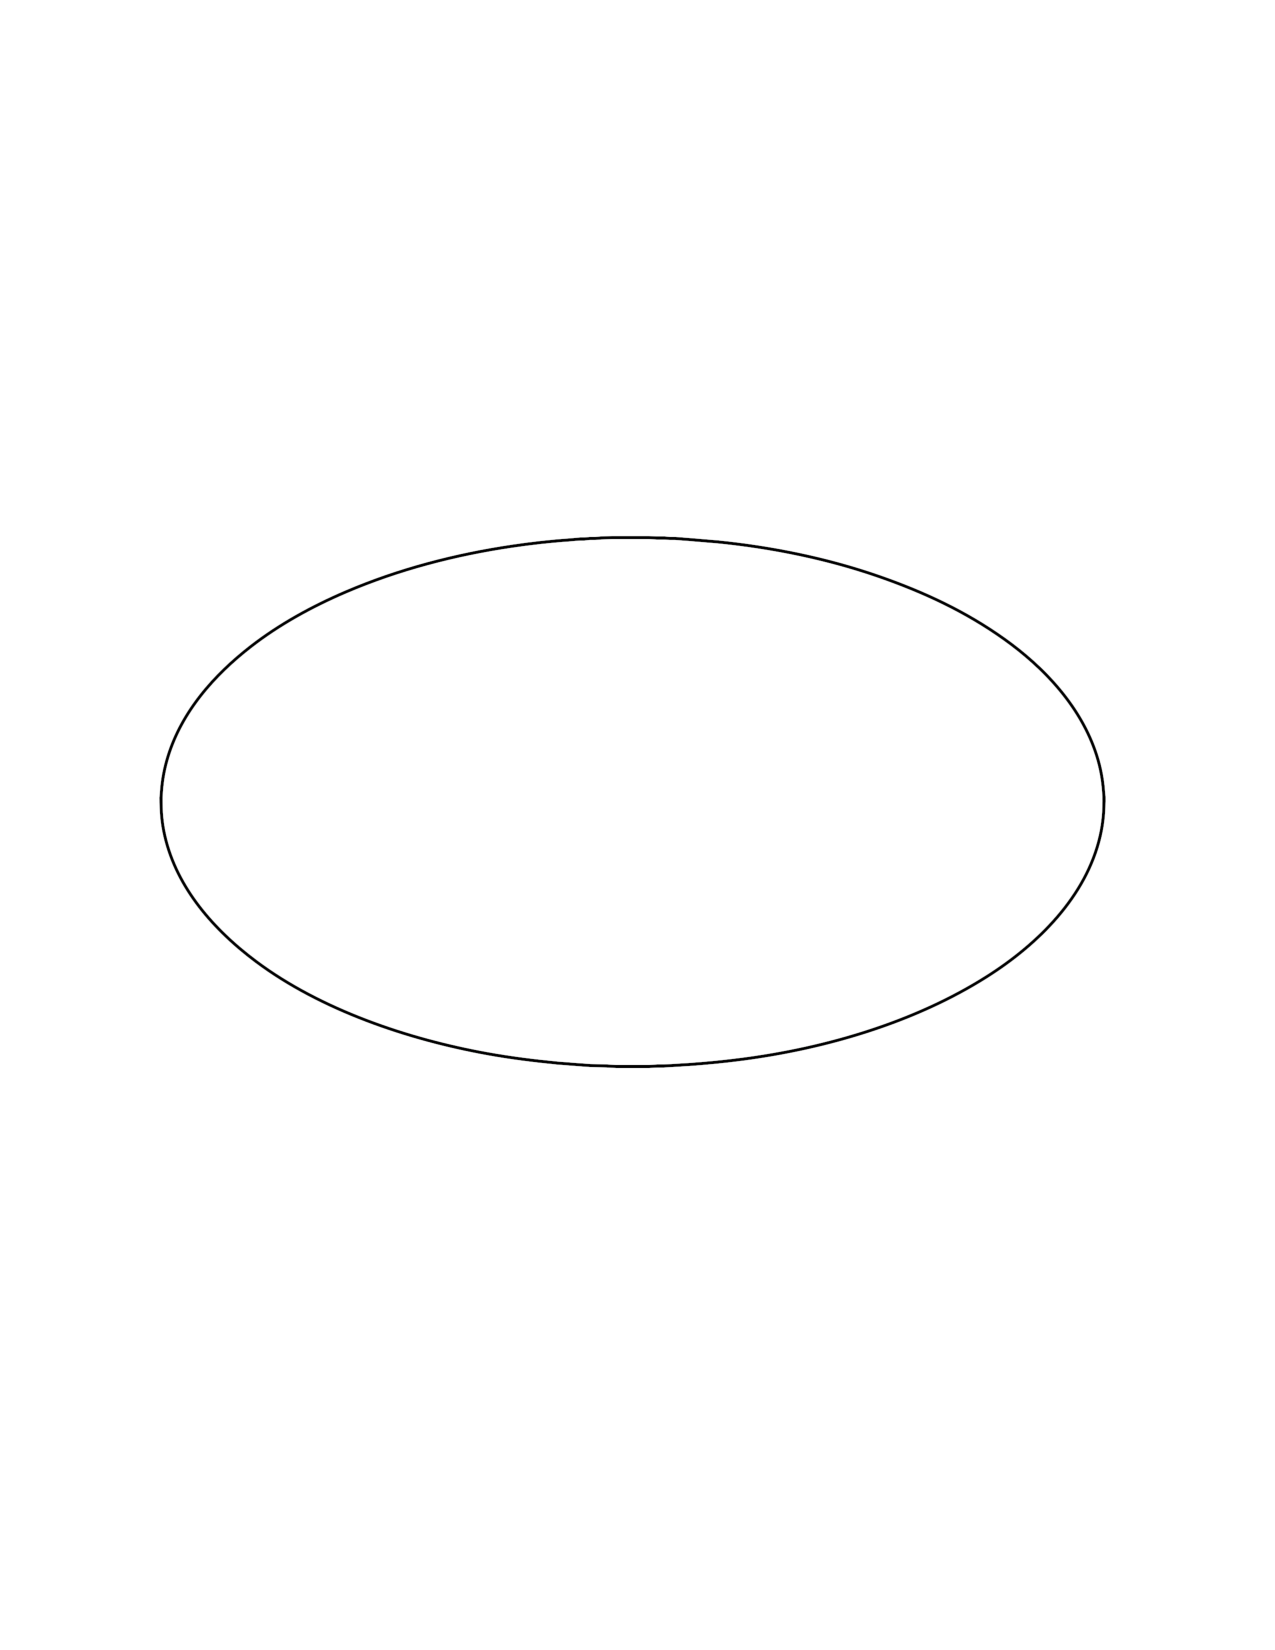
\includegraphics[width=\textwidth]{./images/00ellipse.pdf}};
        \begin{scope}[x={(image.south east)}, y={(image.north west)}]
          \node at (0.3, 0.5) {$N, m$};
          \node at (0.43, 0.58) {$\vec u$};
          \draw [-stealth] (0.4,0.52) -- (0.5,.58);
        \end{scope}
      \end{tikzpicture}
    \end{subfigure}
  \end{figure}


  Let us examine an example of a water in a river.
  Assume that the water has some velocity $\vec {u}$, momentum $\vec{P}$ and also that it can 
  exchange mass and heat, the latter given by $\d Q = T \d S$.
  Therefore an incremental change in the energy of this system can be expressed as
  \begin{displaymath}
    \d E = \vec u \cdot \d \vec P - p \d V + T \d S + \mu \d N,
  \end{displaymath}
  where $\mu$ is the chemical potential of the system.
  Thus
  \begin{displaymath}
    E = E(\vec P, V, S, N).
  \end{displaymath}
  This is the \fndef{energy representation} of a thermodynamical system.
  Comparing the equations above we obtain
  \begin{displaymath}
    \d E = \underbrace{\ptf{E}{\vec P}}_{\vec u} \d \vec P + \underbrace{\ptf{E}{V}}_{- p} \d V 
    + \underbrace{\ptf{E}{S}}_{T} \d S + \underbrace{\ptf{E}{N}}_{\mu} \d N,
  \end{displaymath} % TODO add some explanation about the fact that \ptf{E}{\vec P} = \vec u.
  Those are called the Gibbs relation for $E$.

  If we want to compute it for a fixed entropy we get
  \begin{displaymath}
    \d S = \frac{1}{T} \d E - \frac{\vec u}{T} \d \vec P + \frac{p}{T} \d V - \frac{\mu}{T} \d N.
  \end{displaymath}
  Thus
  \begin{displaymath}
    S = S(E, \vec P, V, N), \quad
    \d S = \underbrace{\ptf{S}{E}}_{\frac{1}{T}} \d E + \underbrace{\ptf{S}{\vec P}}_{- \frac{\vec u}{T}} \d \vec P 
    + \underbrace{\ptf{S}{V}}_{\frac{p}{T}} \d V + \underbrace{\ptf{S}{N}}_{- \frac{\mu}{T}} \d N,
  \end{displaymath}
  Those are Gibbs relations for $S$.

  It is very tricky to control entropy --- it's much easier to control the temperature.
  To obtain a description of our system when $T$ is an independent variable we need to use another thermodynamical potential,
  % switch variables i.e. use other thermodynamical potential.
  which is Helmholz free energy.
  Transition is obtained by
  \begin{displaymath}
    (S \ra T) \quad F = E - TS, \quad F = F(\vec P, V, T, N)
  \end{displaymath}
  \begin{displaymath}
    \d F = - S \d T - p \d V  + \vec{u} \d \vec {P}  + \mu \d N.
  \end{displaymath}
  Now we can do the same to switch other variables. Thus we obtain
  \begin{displaymath}
    (V \ra P) \quad H = E + p V, \quad H = H(\vec P, p, S, N),
  \end{displaymath}
  which is called an enthalpy,
  \begin{displaymath}
    (S \ra T) \quad G = E + pV - TS, \quad G = G(\vec P, p , T, N),
  \end{displaymath}
  which is called a Gibbs potential.

  Now we want to consider if they are Galilean invariant
  % \todo Fig\#4.

  % \begin{figure}[ht]
  %   \centering
  %   \begin{tikzpicture}
  %     \node[anchor=south west] (image) at (0,0)
  %     {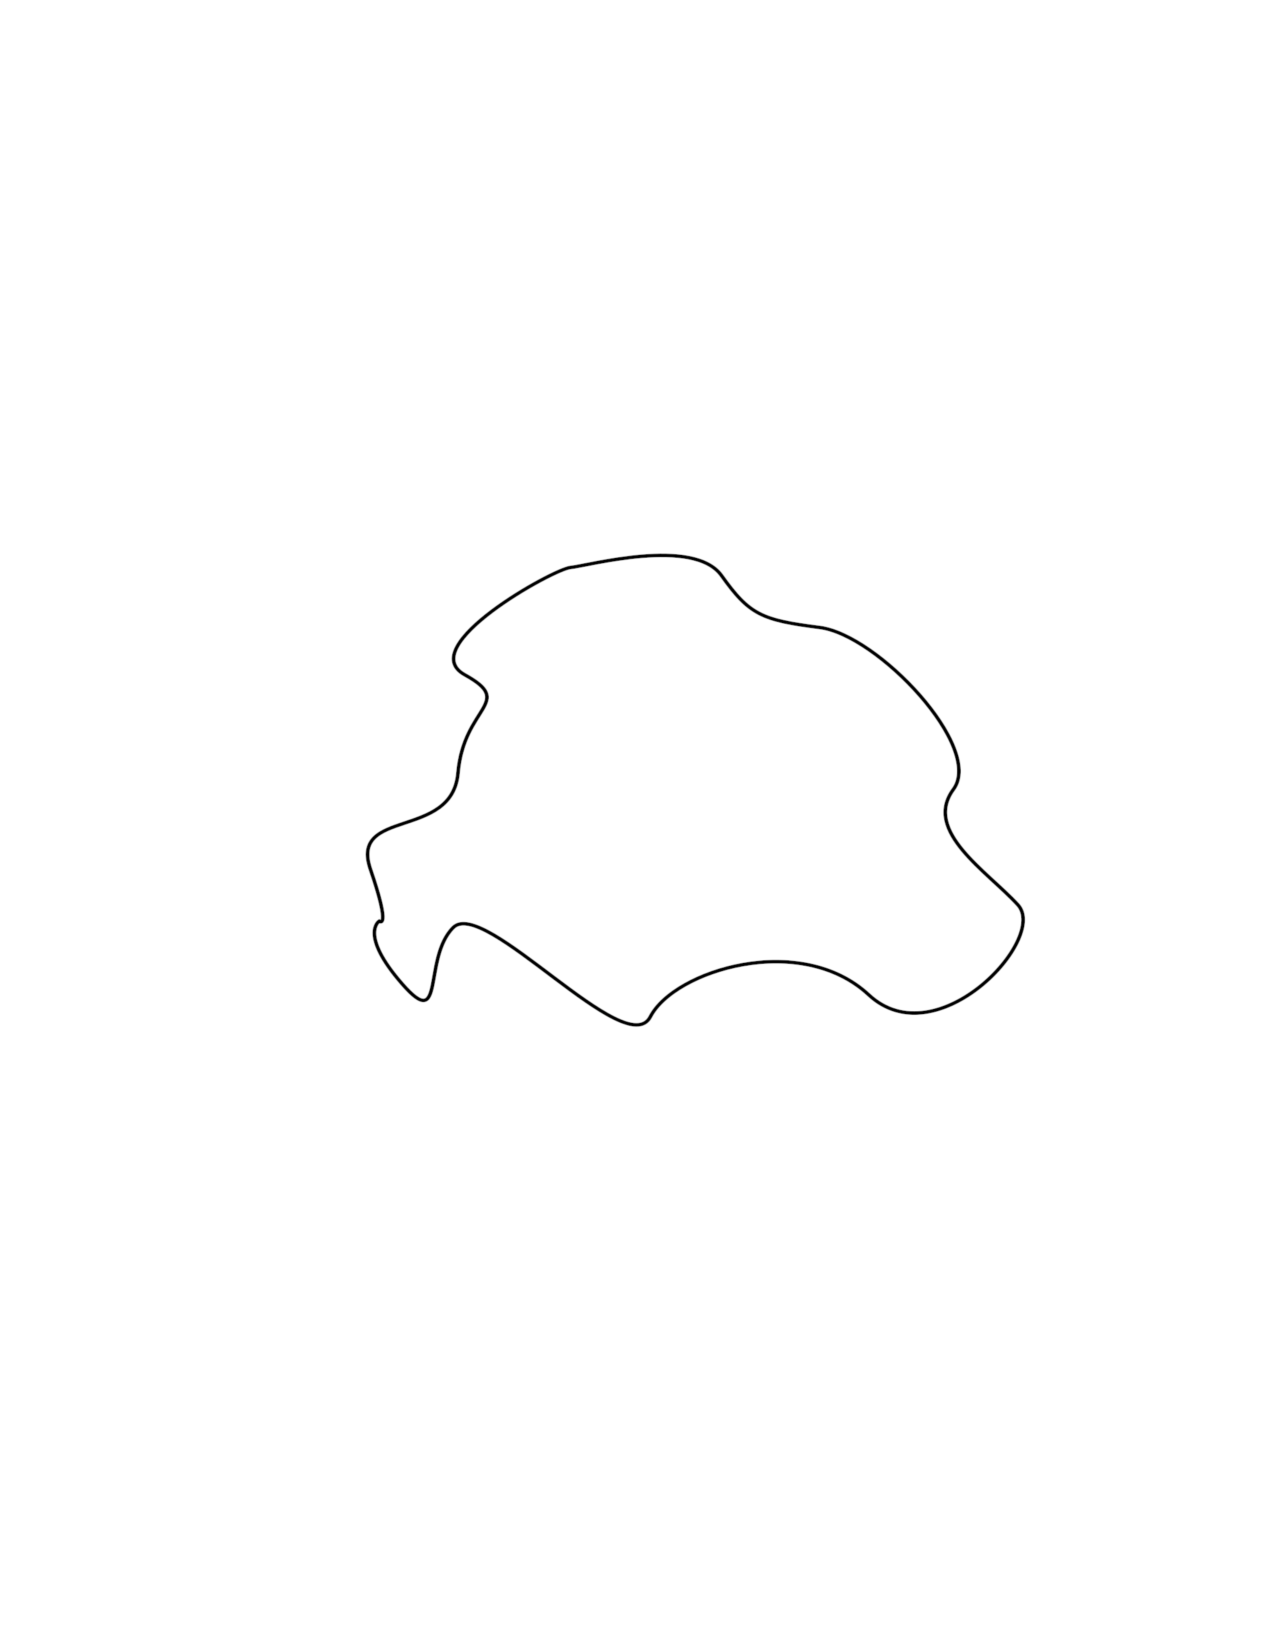
\includegraphics[width=0.5\textwidth]{./images/00splash.pdf}};
  %     \begin{scope}[x={(image.south east)}, y={(image.north west)}]
  %       \node at (0.3, 0.5) {$N, m$};
  %       \node at (0.43, 0.58) {$\vec u$};
  %       \draw [-stealth] (0.4,0.52) -- (0.5,.58);
  %     \end{scope}
  %   \end{tikzpicture}
  % \end{figure}

  \begin{displaymath}
    E(\vec P, V, S, N) = E_0 (V, S, N) + \frac{\vec P^2}{2 M},
  \end{displaymath}
  where $E_0$ is the \fndef{internal energy}.
  For other potentials we obtain
  \begin{displaymath}
    H(\vec P, p , S, N) = H_0(p, S, N) + \frac{\vec P^2}{2 M},
  \end{displaymath}
  \begin{displaymath}
    F(\vec P, V, T, N) = F_0(T, V, N) + \frac{\vec P^2}{2 M},
  \end{displaymath}
  \begin{displaymath}
    G(\vec P, V, T, N) = G_0(T, p, N) + \frac{\vec P^2}{2 M}.
  \end{displaymath}
  
  Using $\vec P = M \vec u$ we get
  \begin{displaymath}
    E = E_0 + \frac{1}{2} M \vec u ^2.
  \end{displaymath}
  \begin{displaymath}
    \d E = \d E_0 + \vec u \cdot \d \vec P,
  \end{displaymath}
  \begin{displaymath}
    \d S = - \frac{1}{T} \vec u \cdot \d \vec P + \frac{1}{T} \d E + \frac{p}{T} \d V - \frac{\mu}{T} \d N,
  \end{displaymath}
  \begin{displaymath}
    \d S = \frac{1}{T}\d E_0 + \frac{p}{T} \d V - \frac{\mu}{T} \d N 
    \qLRa S(\vec P , E , V, N) = S(E_0, V, N).
  \end{displaymath}
  Thus $S$ is a Galilean invariant.

  \subsection{Heterogenous macroscopic system}
  \todo Fig\#5

  \begin{figure}
    \centering
     \begin{tikzpicture}
       \node[anchor=south west] (image) at (0,0)
       {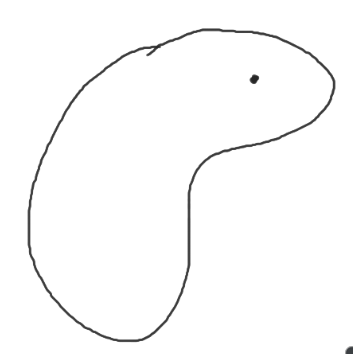
\includegraphics[width=0.25\textwidth]{./images/00Fig5.png}};
       \begin{scope}[x={(image.south east)}, y={(image.north west)}]
         \node at (0.6, 0.7) {$v = \d\vec r$}; % TODO what does it mean XD
         \node at (0.35, 0.15) {$\Omega$}; % TODO what does it mean XD
         \node at (0.95, 0.45) {$\mathbb{M} = \int_\Omega \rho(\vec r, t) \d \vec r$}; % TODO what does it mean XD
         \node at (0.95, 0.25) {$\mathbb{E} = \int_\Omega \epsilon(\vec r, t) \d \vec r$}; % TODO what does it mean XD
       \end{scope}
     \end{tikzpicture}
    \caption{Sample volume $\Omega$. $\rho$ stands for mass density, $\varepsilon$ for density of the system.}
    \label{fig:1.5}
  \end{figure}

  ,,Densities'' are extensive properties per unit volume.
  Assume that $V = \const$, $\d V = 0$.
  Example of densities
  \begin{itemize}
    \item $\rho = \frac{M}{V}$ mass density,
    \item $\vec j = \frac{\vec P}{V}$ momentum density,
    \item $\varepsilon = \frac{E}{V}$ energy density,
    \item $\sigma = \frac{S}{V}$ entropy density.
  \end{itemize}
  \begin{displaymath}
    \d E = \vec u \d \vec P - p \d V + T \d S + \mu \d N / \cdot \frac{1}{V}.
  \end{displaymath}
  \begin{displaymath}
    \d \varepsilon = \vec u \cdot \d \vec j + T \d \sigma + \mu\d n, \quad \d n = \frac{\d \rho}{m},
  \end{displaymath}
  \begin{displaymath}
    \rho = \frac{M}{V} = \frac{Nm}{V} = nm \qLRa \d n = \frac{\d \rho}{m}.
  \end{displaymath}
  Thus the energy fundamental representation in terms of densities can be written as
  \begin{displaymath}
    \varepsilon = \varepsilon(\vec j, \sigma, \rho).
  \end{displaymath}
  After performing a Galilean transform we get
  \begin{displaymath}
    \varepsilon(\vec j, \sigma, \rho) = \varepsilon_0(\sigma, \rho) + \frac{1}{2} \rho \vec u ^2.
  \end{displaymath}
  
  We can do the same to represent entropy in terms of densities
  \begin{displaymath}
    \d S = \dots \frac{1}{V} \qLRa  \d \sigma = \frac{1}{T} \d \varepsilon_0 - \frac{1}{T} \frac{\mu}{m} \d p.
  \end{displaymath}
  Thus
  \begin{displaymath}
    \sigma = \sigma(\varepsilon_0, \rho),
  \end{displaymath}
  which is also Galilean invariant.


  \subsection{Flow of Heterogenous macroscopic system}
  We are using thermodynamics equilibrium despite the fact that the system flows (which means that it is \emph{not} in the equilibrium).
  However there is no contradiction if we assume local, thermodynamical equilibrium.
  The same assumption is made in Navier-Stokes equations.

  From now one we use pseudostatic transition.
  The difference between quasi-static and pseudostatic is that pseudostatic need not to be reversible.
  Forces which acts during quasi-static transformation are those which keeps the system in equilibrium.
  Example of pseudostatic transition which is not quasi-static is a flow of viscose fluid.
  \todo Fig\#6.

  \begin{figure}
    \centering
     \begin{tikzpicture}
       \node[anchor=south west] (image) at (0,0)
       {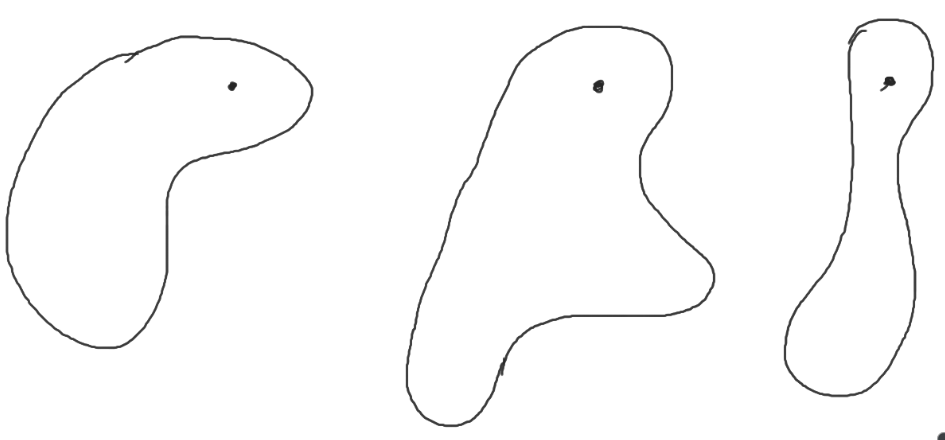
\includegraphics[width=0.45\textwidth]{./images/00Fig6.png}};
       \begin{scope}[x={(image.south east)}, y={(image.north west)}]
         \node at (0.4, 0.9) {$\varepsilon(\vec j, \sigma, p)$}; 
         \node at (0.4, 0.75) {$\sigma(\varepsilon_0, p)$}; 
         \node at (0.2, 0.15) {$\Omega(t_1)$}; 
         \node at (0.6, 0.15) {$\Omega(t_2)$}; 
         \node at (0.9, 0.15) {$\Omega(t_3)$}; 
       \end{scope}
     \end{tikzpicture}
    \label{fig:1.6}
  \end{figure}
  
  
  \subsection{Kinematics}

  We have two descriptions: Eulerian and Lagrangian.
  Transition between them is obtained by
  % (\todo Fig\#7) 

  \begin{figure}
    \centering
     \begin{tikzpicture}
       \node[anchor=south west] (image) at (0,0)
       {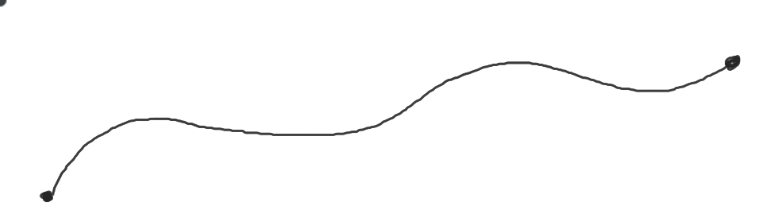
\includegraphics[width=0.25\textwidth]{./images/00Fig7.png}};
       \begin{scope}[x={(image.south east)}, y={(image.north west)}]
         \node at (0.2, 0.1) {$\vec R$}; 
         \node at (0.9, 0.9) {$\vec r(\vec R, t)$}; 
       \end{scope}
     \end{tikzpicture}
    \label{fig:1.7}
  \end{figure}

  

  the solutions to the initial problem
  \begin{displaymath}
    \dfrac{\vec r}{t} = \vec u(r,t), \quad \vec r(t = 0) = \vec R.
  \end{displaymath}

  We want to find dependence of densities as the particle move, and those are
  \begin{center}
    \begin{tabular}{c|c|c|}
      & Euler & Lagrange \\
      \hline
      velocity & $\vec u(r, t) $ & $\vec u[ r(t), t]$\\
      density & $\rho(r, t)$ & $\vec \rho[ r(t), t]$\\
      \hline
    \end{tabular}
  \end{center}
  \begin{displaymath}
    \dfrac{\vec u}{t} = ?, \quad \dfrac{\rho}{t} = ?.
  \end{displaymath}
  
  To do that define $\beta = (\vec u, \rho, S, \sigma, \dots)$. 
  We want to find how $\beta$ change while following the motion 
  of the particle $r(t)$.
  \begin{displaymath}
    \dfrac{\beta}{t} = \dfrac{\beta[\vec r(t),t]}{t} = \ptf{\beta}{t} + \dfrac{r_1 }{t} \ptf{\beta}{r_1} 
    + \dfrac{r_2}{t} \ptf{\beta}{r_2} 
    + \dfrac{r_3}{t} \ptf{\beta}{r_3}  
  \end{displaymath}
  \begin{displaymath}
    = \ptf{\beta}{t} + \vec u (t)\cdot \nabla \beta 
    = \ptf{\beta}{t} + \d \beta(\vec u(t)).
  \end{displaymath}

  \begin{figure}
    \centering
     \begin{tikzpicture}
       \node[anchor=south west] (image) at (0,0)
       {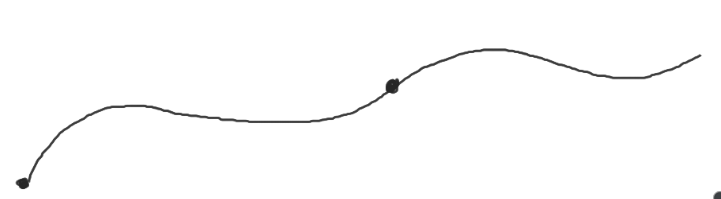
\includegraphics[width=0.25\textwidth]{./images/00Fig8.png}};
       \begin{scope}[x={(image.south east)}, y={(image.north west)}]
         \node at (0.2, 0.1) {$\vec R$}; 
         \node at (0.7, 0.4) {$\beta(\vec r(t), t)$}; 
       \end{scope}
     \end{tikzpicture}
    \label{fig:1.8}
  \end{figure}


  Equation 
  \begin{equation}
    \dfrac{\beta}{t} = \ptf{\beta}{t} + \vec u(t) \cdot \nabla \beta,
    \label{eq:1}
  \end{equation}
  shows a relationship between Eulerian and Lagrangian world, because
  $\dfrac{\beta}{t}$ is a typical Lagrangian while fields (like $\vec u(t)$) are common in Euler's description.
  (Fields are Eulerian objects).
  We introduce a \fndef{total (material) derivative} as 
  \begin{displaymath}
    \dfrac{\dots}{t} = \underbrace{\ptf{\dots}{t}}_{\tm{local derivative}} + \underbrace{\vec u \cdot \nabla(\dots)}_{\tm{advective derivative}}.
  \end{displaymath}
  
  Acceleration of fluid particle
  \begin{displaymath}
    \beta = \vec u \qLRa \dfrac{\beta}{t} = \dfrac{\vec u}{t}.
  \end{displaymath}
  Consider converging chanell with a stationary flow, i.e. $\ptf{\vec u}{t} = 0$.

  % Fig\#9.

  \begin{figure}
    \centering
    \begin{tikzpicture}
      \node[anchor=south west] (image) at (0,0)
      {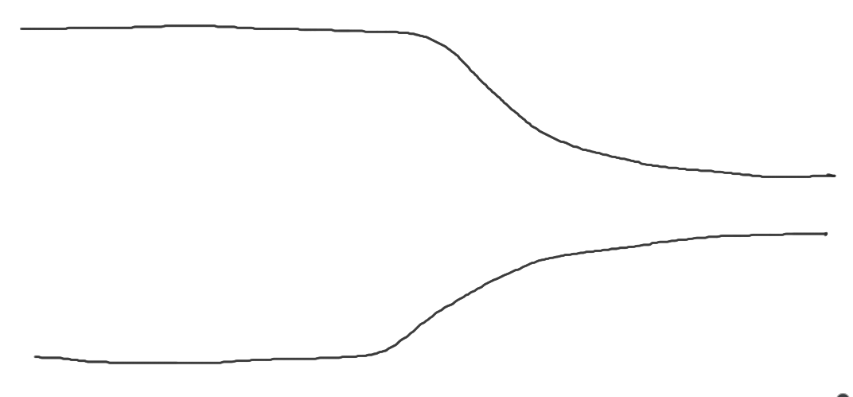
\includegraphics[width=0.25\textwidth]{images/00Fig9.png}};
        \begin{scope}[x={(image.south east)}, y={(image.north west)}]
        \node at (0.1, 0.6) {$\vec v_1$};
        \draw [-stealth] (0.1, 0.5) -- (0.2, 0.5);
        \node at (0.1, 0.3) {$r_1$};

        \node at (0.7, 0.6) {$\vec v_2$};
        \draw [-stealth] (0.7, 0.5) -- (0.9, 0.5);
        \node at (0.7, 0.3) {$r_2$};
        \end{scope}
    \end{tikzpicture}
    \label{fig:1.9}
  \end{figure}

  

  With that in mind
  \begin{displaymath}
    \dfrac{\vec u}{t} = \ptf{\vec u}{t} + \vec u \cdot \nabla \vec u = \vec u \cdot \nabla \vec u.
  \end{displaymath}
  The term $\vec u \cdot \nabla \vec u$ should be interpreted as follows.
  Treat $\vec u$ as a map $\vec u(\vec r): \RR^3 \ra \RR^3$. 
  Thus $\nabla \vec u$ is just a map $D \vec u: \RR^3 \ra \RR^3$ expressed by a matrix
  \begin{displaymath}
    \vec u(\vec r) = \begin{bmatrix}
      u_1 (r_1, r_2, r_3)\\
      u_2 (r_1, r_2, r_3)\\
      u_3 (r_1, r_2, r_3)
    \end{bmatrix}, \quad 
    D \vec u = \begin{bmatrix}
      \ptf{u_1}{r_1} & \ptf{u_1}{r_2} & \ptf{u_1}{r_3} \\
      \ptf{u_2}{r_1} & \ptf{u_2}{r_2} & \ptf{u_2}{r_3} \\
      \ptf{u_3}{r_1} & \ptf{u_3}{r_2} & \ptf{u_3}{r_3}
    \end{bmatrix}.
  \end{displaymath}
  Therefore inner product $\vec u \cdot \nabla \vec u$ really means
  \begin{displaymath}
    \vec u \cdot \nabla \vec u = (D \vec u)(\vec u).
  \end{displaymath}
  At least I think so\dots
  

  
  The term $\vec u \cdot \nabla \vec u$ is called a \fndef{convective acceleration}.
  Although the flow is stationary, the particle experiences acceleration related to movement along the flow lines. 
  
  
  We can interpret the fluid flow as a mapping which takes one point and maps it to the other.

  % Fig\#10.
  \begin{figure}
    \centering
    \begin{tikzpicture}
      \node[anchor=south west] (image) at (0,0)
      {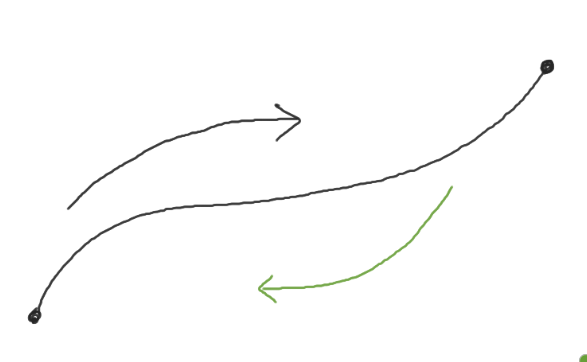
\includegraphics[width=0.35\textwidth]{images/00Fig10.png}};
        \begin{scope}[x={(image.south east)}, y={(image.north west)}]
          \node at (0.3, 0.8) {$r(\cdot)$};
          \node at (0.6, 0.1) {$r^{-1}(\cdot)$};
        \end{scope}
    \end{tikzpicture}
    \label{fig:1.10}
  \end{figure}

  
  
  \paragraph{Streakline}

  \begin{figure}
    \centering
    \begin{tikzpicture}
      \node[anchor=south west] (image) at (0,0)
      {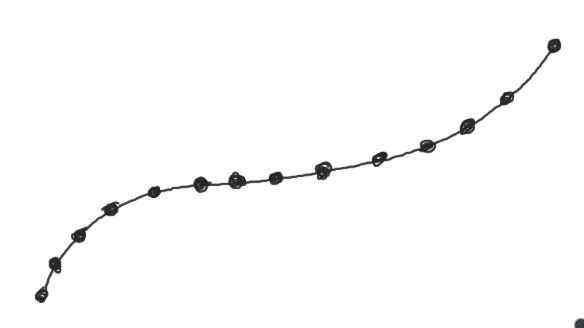
\includegraphics[width=0.25\textwidth]{images/00Fig11.png}};
        \begin{scope}[x={(image.south east)}, y={(image.north west)}]
          \node at (0.0, 0.2) {$\vec y$};
          \node at (0.8, 0.9) {$\vec r(\vec y, t)$};
        \end{scope}
    \end{tikzpicture}
    \caption{Streakline is a line made of all particles that for time $s$, $0 \leq s \leq t$ 
    passed through a fixed point $\vec y$.}
    \label{fig:1.11}
  \end{figure}

  

  Imagine a cigarette and assume that there is no diffusion. 
  The smoke is made out of small, fluid particles.
  The flow line is made out of fluid particles which were passing through $\vec y$ in the time interval
  $0 \leq s \leq t$.
  Suppose that we froze time at $t = t_0$.
  Choose point $A$.
  \fndef{Streakline} through the point $A$ is a curve made of all particles (in the given moment) that have passed
  through the point $A$ at some $t < t_0$.
  \begin{displaymath}
    \vec r [ \vec R(y,s), t], \quad 0 \leq s \leq t.
  \end{displaymath}

  \paragraph{Streamline}
  Streamline is a integral curve of a vector field $X(t)$ at a given time $t = t_0$.
  They do not intersect neither with each other nor with themselves.
  Equation:
  \begin{displaymath}
    \dfrac{r}{s} = \vec u(\vec r, t).
  \end{displaymath}

  \paragraph{Trajectory}
  \fndef{Trajectory} is a path traced by a chosen particle.

  For the stationary flow the streakline and streamline are the same.
  
  For stationary flows i.e. $(\ptf{u}{t} = 0)$.
  Trajectory $\equiv$ streakline $\equiv$ streamline.

  \section{Balance equations}
  $\vec u(\vec r, t)$ --- velocity field, $\rho(\vec r, t)$ --- density flow.
  They are not completely independent since the mass has to be conserved.
  % \todo Fig\#13

  \begin{figure}
    \centering
    \begin{tikzpicture}
      \node[anchor=south west] (image) at (0,0)
      {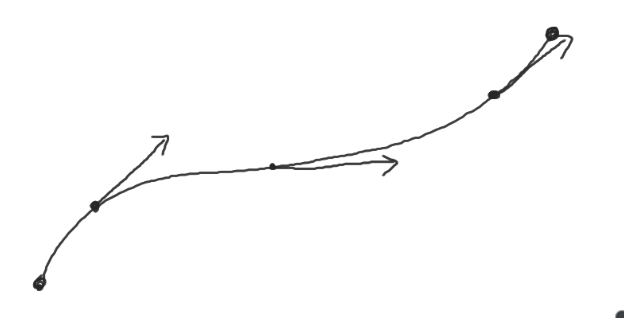
\includegraphics[width=0.35\textwidth]{images/00Fig12.png}};
    \end{tikzpicture}
    \caption{Streamline is just a flow of a vector field for at a fixed time $t$.}
    \label{fig:1.12}
  \end{figure}
  
  \begin{displaymath}
    M = \int_V \rho(\vec r, t) \d \vec r,
  \end{displaymath}
  \begin{displaymath}
    \ptf{M}{t} = \ptf{}{t} \in V \rho(\vec r, t) = \int_V \ptf{\rho(\vec r, t)}{t} \d \vec r.
  \end{displaymath}
  \begin{displaymath}
    \ptf{M}{t} = \int_V \ptf{\rho}{t} \d \vec r
    = -\int_{\partial V} \rho \vec u \cdot \vec n \d a,
  \end{displaymath}
  using Stokes theorem
  \begin{displaymath}
    = - \int_V \nabla \cdot (\rho \vec u)  \d \vec r.
  \end{displaymath}

  In other words
  \begin{displaymath}
    \int_V \left[ \ptf{\rho}{t} + \nabla \cdot (\rho \vec u) \right] \d \vec r = 0 ,
  \end{displaymath}
  and, since $V$ is arbitrary,
  \begin{displaymath}
    \ptf{\rho}{t} + \nabla \cdot (\rho \vec u) = 0.
  \end{displaymath}
  Which is called the \fnvi{continuity equation}.
  This is the general mass conservation, fluid can change density and so on.



  \chapter{Lecture 2}
  \paragraph{Reminder}
  Material derivative 
  \begin{displaymath}
    \dfrac{}{t} = \frac{D}{Dt} = \ptf{}{t} + \vec u \cdot \nabla \cdot
  \end{displaymath}

  Mass conservation implies the continuity equation
  \begin{displaymath}
    \ptf{\rho}{t} + \nabla \cdot ( \rho \vec u ) = 0.
  \end{displaymath}

  \paragraph{New stuff}
  Expanding the above equation we obtain
  \begin{displaymath}
    \underbrace{\ptf{\rho}{t} + \vec u \cdot \nabla \rho}_{\dfrac{\rho}{t}} + \rho \nabla \cdot \vec u = 0,
  \end{displaymath}
  and thus
  \begin{displaymath}
    \frac{1}{\rho} \dfrac{\rho}{t} = - \nabla \cdot \vec u.
  \end{displaymath}
  If we introduce \fndef{specific volume} $\nu = 1 / \rho$ we obtain
  \begin{displaymath}
    \frac{1}{\nu} \dfrac{\nu}{t} = \nabla \cdot \vec u.
  \end{displaymath}

  We introduced that because we want to study incompressible flow.
  If the flow is incompressible we express it by saying that
  \begin{displaymath}
    \dfrac{\rho}{t} = 0 \quad \tm{or}\quad  \dfrac{\nu}{t} = 0.
  \end{displaymath}
  From the continuity equation incompressibility of the flow implies that
  \begin{displaymath}
    \nabla \cdot \vec u = 0.
  \end{displaymath}
  
  For the incompressible flow the $\vec u$ is divergence-free or solonoidal (\todo I didn't hear it right).

  If $\nabla \cdot \vec u = 0$ and $ f(\vec r, t) = f_0 = \tm{const}$ then
  \begin{displaymath}
    \forall t \quad f(\vec r, t) = f_0 = \tm{const}.
  \end{displaymath}

  Positive divergence implies expansion, negative implies compression.
  

  \section{Newton's second law (Momentum balance)}
  \fndef{Material volume}. Consider closed system (volume $V(t)$) which is comprised of the same fluid particles.
  It flows with a fluid. \todo Fig0.
  We want to calculate the momentum of such \fndef{material volume}.
  It is obviously an integral
  \begin{displaymath}
    \vec P (t) = \int_{V(t)} \rho(\vec r, t) \vec u(\vec r, t) \d \vec r.
  \end{displaymath}
  That is a linear momentum of the material volume.
  We want to state the Newton second law:
  \begin{displaymath}
    \dfrac{\vec P(t)}{t} = \vec F, 
  \end{displaymath}
  where $\vec F$ is a net force.
  \begin{displaymath}
    \dfrac{\vec P}{t} = \dfrac{}{t} \int_{V(t)} \rho(\vec r, t) \vec u (\vec r, t) \d \vec r = ?.
  \end{displaymath}
  
  Here is a theorem (i.e. fancy name for Leibniz rule):
  
  \begin{theorem}[Raynold's transport theorem]
    \begin{displaymath}
      \dfrac{}{t} \int_{V(t)} \beta (\vec r, t) \d \vec r = 
      \int_{V}\left[ \ptf{\beta}{t} + \nabla \cdot (\beta \vec u) \right] \d \vec r
      = \int_V \left[ \ptf{\beta}{t} + \vec u \cdot \vec \beta + \beta \nabla \cdot \vec u \right]
      ,
    \end{displaymath}
    where $V$ is a fixed quantity, called control volume (i.e. any volume that coincides with $V(t)$).
  \end{theorem}

  The things that contribute to this change can be interpreted as
  \begin{enumerate}
    \item local change $\ptf{\beta}{t}$,
    \item advection i.e. $\vec u \cdot \nabla \beta$,
    \item changing volume i.e. $\beta \nabla\cdot \vec u$.
  \end{enumerate}

  Using it to the momentum we get
  \begin{displaymath}
    \dfrac{\vec P }{t} = \dfrac{}{t} \int_{V(t)} \rho \vec u \d \vec r 
    = \int_V \left[ \ptf{\rho\vec u }{t} + \nabla \cdot (\rho \underbrace{\vec u \vec u}_{\vec u \otimes \vec u}) \right]
  \end{displaymath}
  
  \paragraph{Homework} Show that if $\beta = \rho b$, then 
  \begin{displaymath}
    \dfrac{}{t} \int_{V(t)} \rho b \d \vec r = \int_{V} \rho \dfrac{b}{t} \d \vec r,
  \end{displaymath}
  using RTT (Raynold's transport theorem) and the continuity equation.
  
  \begin{displaymath}
    \dfrac{\vec P}{t} = \dfrac{}{t} \int_{V(t)} \rho \vec u \d \vec r 
    = \int_V \rho \dfrac{\vec u}{t} \d \vec r 
    = \vec F,
  \end{displaymath}
  and thus the integral's form of Newton second law
  \begin{displaymath}
    \int_V \rho \dfrac{\vec u}{t} \d \vec r = \vec F.
  \end{displaymath}
  
  \section{Further consequences of RTT}
  \todo Fig1.
  
  \begin{displaymath}
    M = \int_V \rho \d \vec r \qLRa \ptf{M}{t} 
    = \ptf{}{t} \int_V \rho \d \vec r 
    = \int_V \ptf{\rho}{t} \d \vec r 
    = - \int_{\partial V} \rho \vec u \cdot \hat n \d S 
    = - \int_V \nabla \cdot (\rho \vec u) \d \vec r.
  \end{displaymath}

  To note: material volume is the volume that flows with the fluid.
  
  \todo Fig2

  Consider material volume $V(t)$ and its mass given by
  \begin{displaymath}
    M = \int_{V(t)}  \rho \d \vec r.
  \end{displaymath}
  Thus the mass conservation means that
  \begin{displaymath}
    \dfrac{M}{t} = 0.
  \end{displaymath}

  We calculate
  \begin{displaymath}
    \dfrac{M}{t} = \dfrac{}{t} \int_{V(t)} \rho \d \vec r 
    = \int_V \left[ \ptf{\rho}{t} + \nabla \cdot (\rho \vec u) \right]\d \vec r 
    = 0.
  \end{displaymath}
  
  In the following equation
  \begin{displaymath}
    \int_V \rho \dfrac{\vec u}{t} \d \vec r = \vec F,
  \end{displaymath}
  we do not know what $\vec F$ is and therefore need a model for it.

  \todo Fig3

  Consider that the fluid acts on its surface element $\d a$ (with normal vector $\hat n$).
  Let $\vec t$ be a force per unit area, and $\d \vec F = \vec t \d a$.
  \begin{displaymath}
    \vec F \os{\tm{model}}{=} \int_{\partial V} \d \vec F 
    = \int_{\partial V}  \vec t \cdot \d a
    = - \int_V \nabla p \d \vec r.
  \end{displaymath}
  Assume that $\vec t = - p \hat{n}$, where $p $ is a pressure and $\nabla p $ a \fndef{pressure field}.
  
  \begin{displaymath}
    \int_V \rho \dfrac{\vec u }{t} = \d \vec r = - \int_V \nabla p \d \vec r,
  \end{displaymath}
  \begin{displaymath}
    \int_V \left[ \rho \dfrac{\vec u}{t} + \nabla p \right]\d \vec r = 0 
    \qLRa \rho \dfrac{ \vec u }{t} = - \nabla p.
  \end{displaymath}
  We may also write it as 
  \begin{displaymath}
    \rho \left( \ptf{\vec u}{t} + \vec u \cdot \nabla \cdot \vec u  \right) = - \nabla p.
  \end{displaymath}
  This is the \fnvi{Euler model of the ideal fluid} (ideal fluid without dissipation).
  
  \section{Equilibrium}
  Equilibrium is obtained when $\vec u = 0$ and thus $\nabla p = 0$.
  Especially if $p = \const$.
  \begin{itemize}
    \item ideal fluid $ \vec t = - p \hat n$
    \item In general $ \vec t = \Sigma^T \cdot \vec n$, where $\Sigma$ is \fndef{Cauchy stress tensor} (second order tensor).
  \end{itemize}
  In general case force can have a 
  
  \begin{displaymath}
    \ul{\ul{\Sigma}} = - p \ul{\ul{1}} + \ul{\ul{\Sigma'}} % TODO that's not all correct. 
  \end{displaymath}


  \begin{displaymath}
    \vec F = \int_{\partial V} \vec t \d a = \int_{\partial V} \Sigma^T \cdot \hat n \d a = \int_V \nabla \cdot \Sigma \d \vec r.
  \end{displaymath}
  Newton's second law
  \begin{displaymath}
    \int_V \rho \dfrac{\vec u}{t} \d \vec r = \nabla \cdot \Sigma \d \vec r.
  \end{displaymath}

  \begin{displaymath}
    \Sigma = \underbrace{- p \ul{\ul{1}}}_{\tm{ideal term}} + \underbrace{\ul{\ul{\Sigma}}}_{\tm{deviatory part}}
  \end{displaymath}
  Deviatoric part vanishes in equilibrium.

  Ideal fluid model $\Sigma' = 0$, $\Sigma = - p \ul{\ul{1}}$.
  \begin{displaymath}
    \nabla \cdot \Sigma = \nabla \left( - p \ul{\ul{1}} \right) = - \nabla p.
  \end{displaymath}

  \paragraph{Summary}
  Til now we formulated
  
  \begin{itemize}
    \item 
      \begin{displaymath}
          \ptf{\rho}{t} + \nabla \cdot ( \rho \vec u ) = 0
      \end{displaymath}
    \item \begin{displaymath}
        \rho \left( \ptf{\vec u }{t} + \vec u \cdot \nabla \cdot \vec u  \right) = \nabla \cdot \Sigma
    \end{displaymath}
  \item What's next?
  \end{itemize}

  \section{Angular momentum}
  Fig4

  Consider material volume $V(t)$, density $\rho$ and a point at $\vec r$ moving with a velocity $\vec u$.
  \begin{displaymath}
    \vec L (t) = \int_{V(t)}\vec r \times \rho \vec u \d \vec r
    = \int_{V(t)} \rho (\vec r \times \vec u) \d \vec r,
  \end{displaymath}
  where $\vec l = \vec r \times \vec u $ is the \fndef{angular momentum per unit mass}.

  The law of the change of the angular momentum
  \begin{displaymath}
    \dfrac{ \vec L }{t} = \vec N,
  \end{displaymath}
  where $\vec N$ is a \fndef{net torque} acting on $V(t)$.
  \begin{displaymath}
    \dfrac{\vec L}{t} = \dfrac{}{t} \int_{V(t)} \rho \vec l \d \vec r \os{\tm{RTT + cont}}{=\joinrel=} \int_V \rho \dfrac{\vec l}{t} \d \vec r.
  \end{displaymath}
  We calculate $\vec N$ by
  \begin{displaymath}
    \vec N = \int_{\partial V} \vec r \times\vec t \d a.
  \end{displaymath}

  \begin{displaymath}
    \int_V \rho \dfrac{\vec l}{t} \d \vec r = \int_V \vec r \times \vec t \d a 
    = \int_{\partial V} (\vec r \times \Sigma^T) \cdot \hat n \d a 
  \end{displaymath}
  using divergence theorem
  \begin{equation}
    = \int_V \nabla \cdot \left[ ( \vec r \times \Sigma^T)^T \right] \d \vec r.
    \label{eq:prev}
  \end{equation}

  where divergence theorem:
  \begin{displaymath}
    \int_{\partial V} T \cdot \hat n \d a = \int_V \nabla \cdot T^T  \d \vec r.
  \end{displaymath}

  Going back to \ref{eq:prev}
  \begin{displaymath}
     = \int_V \left[ \vec r \times \nabla \cdot \Sigma - 2 \vec \sigma \right] \d \vec r,
  \end{displaymath}
  where $\vec \sigma $ is the axial vector associated with $\Sigma$.
  Thus
  \begin{displaymath}
    \int_V \rho \dfrac{ \vec l}{t} \d \vec r = \int_V \left[ \vec r \times \nabla \cdot \Sigma - 2 \vec \sigma \right] \d \vec r ,
  \end{displaymath}
  and since the volume $V$ can be anything we get
  \begin{equation}
    \rho \dfrac{ \vec l }{t} = \vec r \times \nabla \cdot \Sigma - 2 \vec \sigma.
    \label{eq:2.2}
  \end{equation}

  This is too complicated, we need to simplify it.
  
  \begin{displaymath}
    \rho \dfrac{ \vec l }{t} = \rho \dfrac{\vec r \times \vec u}{t} 
    = \rho \vec r \times \dfrac{\vec u}{t} + \rho \dfrac{ \vec r }{t} \times \vec u
    = \vec r \times \underbrace{\rho \dfrac{\vec u}{t}}_{\nabla \Sigma} 
    = \vec r \times \nabla \cdot \Sigma.
  \end{displaymath}

  Substituting it to  \ref{eq:2.2} we get
  \begin{displaymath}
    \vec \sigma = 0.
  \end{displaymath}
  Thus the $\Sigma $ is symmetric.

  The stress tensor need not to be symmetric for magnetic fluids (it works for the simple fluids).


  \paragraph{,,Complex'' fluids}
  \todo Fig5

  Consider a magnetic fluid in a bottle, with magnetic dipoles.
  Assume that we apply a magnetic field, so there is a reorientation and the \fndef{internal torque} appears.
  
  \begin{displaymath}
    \vec N = \int_{\partial V} \vec r \times \vec t \d a + \int_{V} \vec b \d \vec r,
  \end{displaymath}
  where $\vec b$ is the internal torque.
  
  
  \section{Energy conservation}
  \todo Fig6 

  Consider material volume $V$ and a small surface element $\d a$.
  The energy is given by 
  \begin{displaymath}
    E(t) = \int_{V (t)} \rho (\vec r ,t ) e (\vec r, t) \d \vec r ,
  \end{displaymath}
  where $e (\vec r, t)$ is the energy for unit volume.

  The ,,law'' of change
  \begin{displaymath}
    \dfrac{E}{t} = \dfrac{W}{t} + \dfrac{Q}{t},
  \end{displaymath}
  where $W$ is a mechanical work and $Q$ is a heat.

  Using RTT and continuity we get
  \begin{displaymath}
    \dfrac{E}{t} = \dfrac{}{t} \int_{V(t)} \rho e \d \vec r = \int_V \rho \dfrac{e}{t} \d \vec r,
  \end{displaymath}
  
  \begin{displaymath}
    \dfrac{W}{t} = \int_{\partial V } \vec t \d a \cdot \vec u 
    = \int_{\partial V} (\Sigma^T \cdot \vec u ) \cdot \hat n  \d a 
    = \int_V \nabla \cdot ( \ul{\ul{\Sigma}} \cdot u) \d \vec r.
  \end{displaymath}

  \begin{displaymath}
    \dfrac{Q}{t} = - \int_{\partial V} \vec q \cdot  \hat n \d a = - \int_V \nabla \cdot \vec q \d \vec r,
  \end{displaymath}
  where $\vec q$ is the heat flow per unit surface per unit time. % TODO upewnić się, że to jest rzeczywiście to 

  Summing up we get
  \begin{equation}
    \rho \dfrac{ e}{t} = \nabla \cdot ( \Sigma \cdot \vec u) - \nabla \cdot \vec q.
    \label{eq:2.3}
  \end{equation}

  Let's introduce the separation 
  \begin{displaymath}
    e = e_0 + \frac{1}{2} \vec u^2.
  \end{displaymath}

  Substituting it into \ref{eq:2.3} we obtain
  \begin{displaymath}
    \rho \dfrac{e_0}{t} = - \rho \dfrac{}{t} \left( \frac{1}{2} \vec u^2 \right) + \nabla \cdot (\Sigma \cdot \vec u ) - \nabla \cdot \vec q.
  \end{displaymath}
  \begin{displaymath}
    \rho \dfrac{}{t} \left( \frac{1}{2} \vec u ^2  \right) 
    = \vec u \cdot \rho \dfrac{\vec u}{t} 
    = \vec u \cdot ( \nabla \cdot \Sigma) 
    = \nabla \cdot ( \Sigma \cdot u) - \Sigma :\nabla \vec u % TODO Double contraction of tensors
  \end{displaymath}
  
  For the internal energy $e_0$:
  \begin{displaymath}
    \rho \dfrac{e_0}{t} = \Sigma : \nabla \vec u - \nabla \cdot \vec q.
  \end{displaymath}
  
  For $\Sigma = - p \ul{\ul{1}} + \Sigma'$
  \begin{displaymath}
    \Sigma : \nabla \vec u = - p ( \nabla \cdot \vec u) + \Sigma' : \nabla \vec u.
  \end{displaymath}
  
  \section{Ideal fluid approximation}
  We assume no deviatoric stress, and no heat flows
  \begin{align*}
    \Sigma' = 0 \\
    \vec q = 0.
  \end{align*}
  The for the ideal fluid
  \begin{displaymath}
    \rho \dfrac{e_0}{t} = - p ( \nabla \cdot \vec u).
  \end{displaymath}

  This approximation is a result of assuming that the particles move all together, so there is no viscosity and also no way to conduct heat.
  
  For a compressible flow
  \begin{itemize}
    \item $\nabla \cdot \vec u > 0 \qLRa \dfrac{e_0}{t} < 0 $ (expansion),
    \item $\nabla \cdot \vec u < 0 \qLRa \dfrac{e_0}{t} > 0 $ (compression),
  \end{itemize}
  and for the incompressible flow there is no way to change internal energy, $\dfrac{e_0}{t} = 0$.
  In ideal fluid there is no dissipation.
  However the real fluids do.

  \section{Entropy balance} 
  
  \todo Fig7

  Consider closed system and assume that a heat has been transfered to the system.
  We can move between $S$ and $S + \d S$ by reversible and irreversible paths.
  For the reversible one we have 
  \begin{displaymath}
    \d S  = \frac{\d Q}{T},
  \end{displaymath}
  and for irreversible proces
  \begin{displaymath}
    \d S \geq \frac{\d Q}{T}.
  \end{displaymath}
  
  \begin{displaymath}
    S(t) = \int_{V(t)} \rho( \vec r , t) s( \vec r, t) \d \vec r,
  \end{displaymath}
  where $s(\vec r, t)$ is entropy per unit volume.
  Entropy balance implies
  \begin{displaymath}
    \dfrac{S}{t} = \frac{\d_e S}{\d t} + \frac{\d_i S}{\d t} 
  \end{displaymath}
  \begin{displaymath}
    \d_e S = \frac{\d Q}{T}.
  \end{displaymath}
  \begin{displaymath}
    \dfrac{S}{t} = \dfrac{}{t} \int_{V(t)} \rho s \d \vec r = \int-V \dfrac{s}{t} \d \vec r,
  \end{displaymath}
  \begin{displaymath}
    \dfrac{_e S}{t} = - \int_{\partial V} \frac{ \vec q}{T} \cdot \hat n \d a 
    = - \int_V \nabla \cdot \left( \frac{\vec q}{T} \right) \d \vec r
  \end{displaymath}
  \begin{displaymath}
    \dfrac{_i S}{t} = \int_V \theta \d \vec r,
  \end{displaymath}
  where $\theta$ is the entropy production per unit volume per unit time.
  Thus the \fnte{entropy balance equation} is
  \begin{displaymath}
    \rho \dfrac{s}{t} = - \nabla \cdot \left( \frac{\vec q }{T}  \right) + \theta, \quad \theta \geq 0.
  \end{displaymath}

  For ideal fluid (no internal efects) $\theta = 0$, and the change of entropy
  \begin{displaymath}
    \dfrac{s}{t} = 0.
  \end{displaymath}


  \chapter{Lecture 3}

  Recall
  \begin{displaymath}
    \ptf{\rho}{t} + \nabla \cdot (\rho \vec u) = 0,  
    \quad \frac{1}{\nu} \dfrac{\nu}{t} = \nabla \cdot \vec u, 
    \quad \nu = \frac{1}{\rho},
  \end{displaymath}
  \begin{displaymath}
    \rho \dfrac{\vec u }{t} = \rho \left(  \ptf{\vec u}{t} + \vec u \cdot \vec u \right) = \nabla \cdot \Sigma  + \rho g,
  \end{displaymath}
  angular momentum balance
  \begin{displaymath}
    \Sigma^T = \Sigma.
  \end{displaymath}
  energy per unit mass
  \begin{displaymath}
    \rho \dfrac{e_0}{t} = - p (\nabla \cdot \vec u) + \Sigma' : \nabla \vec u - \nabla \cdot \vec q
  \end{displaymath}
  entropy per unit mass
  \begin{displaymath}
    \rho \dfrac{s}{t} = - \nabla \cdot \left( \frac{\vec q }{T} \right) + \theta,
  \end{displaymath}
  where $\theta$ is \fndef{entopy production}. The second law of thermodynamics says that $\theta > 0 $.

  Those are complete system of balance equations and in fact quite general ones.

  \paragraph{Local thermodynamics equilibrium approximation}
  \begin{displaymath}
    \theta = \rho \dfrac{s}{t} + \nabla \cdot \left( \frac{\vec q}{T} \right),
  \end{displaymath}
  \begin{displaymath}
    s = s(e_0, \nu),
  \end{displaymath}
  and the Gibbs relation
  \begin{displaymath}
    \d s = \frac{1}{T}\d e_0 + \frac{p}{T} \d \nu.
  \end{displaymath}
  $\d e_0/\d t$ comes form a flow of a energy and the $\d \nu / \d t$ part comes from continuity equation.
  We can write it as
  \begin{displaymath}
    \rho \dfrac{s}{t} = \frac{1}{T} \underbrace{\rho \dfrac{e_0}{t}}_{\tm{eq } 4} 
    + \frac{p}{T} \underbrace{\frac{1}{\nu} \dfrac{\nu }{t}}_{\tm{eq } 1}.
  \end{displaymath}
  Thus
  \begin{displaymath}
    \rho \dfrac{s}{t} = \frac{1}{T} \left[ - p (\nabla \cdot \vec u) + \Sigma' : \nabla \vec u - \nabla \cdot \vec q \right]
    + \frac{p}{T} (\nabla \cdot \vec u).
  \end{displaymath}
  \begin{displaymath}
    \nabla \cdot \left( \frac{\vec q }{T} \right) = \frac{1}{T} \nabla \cdot \vec q - \frac{1}{T^2} \vec q \cdot \nabla T,
  \end{displaymath}
  \begin{displaymath}
    \theta = - \frac{p}{T} (\nabla \cdot \vec u) + \frac{1}{T} \Sigma' : \nabla \vec u - \frac{1}{T} \nabla \cdot \vec q
    + \frac{p}{T} (\nabla \cdot \vec u) + \frac{1}{T} \nabla \cdot \vec q - \frac{1}{T^2} \vec q \cdot \nabla T.
  \end{displaymath}
  Thus the entropy production is given by the formula
  \begin{displaymath}
    \theta = - \frac{1}{T^2} \underbrace{\vec q \cdot \nabla T}_{\tm{,,force''}} + \frac{1}{T} \underbrace{\Sigma' : \nabla \vec u}_{\tm{,,force}} \geq 0.
  \end{displaymath}
  Imagine that you have a flow and a temperature gradient --- then the fluid will flow from the hotter part to the colder.
  Note that both terms have to be positive, because when one is missing, the other one must be non-negative.

  How does those equations simplify in the ideal fluid model?

  \section{Ideal fluid model}

  Recall that for the ideal fluid we have
  \begin{displaymath}
    \vec q = 0, \quad \Sigma' = 0 \qLRa \theta = 0,
  \end{displaymath}
  and therefore there is no entropy production.

  Hydrodynamics of ideal fluids:
  \begin{enumerate}
    \item $\ptf{\rho}{t} + \nabla \cdot (\rho \vec u) = 0$,
    \item $\rho \dfrac{\vec u}{t} = - \nabla p + \rho \vec g$,
    \item $ \rho \dfrac{e_0}{t} = - p(\nabla \cdot \vec u)$,
    \item $\dfrac{s}{t} = 0$.
  \end{enumerate}
  Since the 2\textsuperscript{nd} is a vector one we have $6$ equations, but, unfortunately 7 variables.
  The one that is missing is the thermodynamical equation of state (for pressure).

  \section{Thermodynamics}
  \begin{displaymath}
    e_0 = e_0(s , \nu)
  \end{displaymath}
  the specific volume is not that interesting, thus we shall use another thermodynamical potential.
  Thus we will use enthalpy
  \begin{displaymath}
    h_0 = e_0 + p \nu = e_0 + \frac{p}{\rho}, \quad h_0 = h_0(s, p), 
  \end{displaymath}
  \begin{displaymath}
    \d h_0 = T \d s + \nu \d p = \underbrace{T\d s}_{ = 0} + \frac{\d p}{\rho}.
  \end{displaymath}
  Thus 
  \begin{displaymath}
    \d h_0 = \frac{\d p}{\rho}, \quad h_0 = h_0(p),\quad \ptf{h_0}{p}|s = \frac{1}{\rho}.
  \end{displaymath}
  Therefore $\rho = \rho(p)$ or $p = p(\rho)$ and that is our missing equation.
  It is called the \fnte{equation of state}.
  
  \paragraph{Ideal gas}
  \begin{displaymath}
    p(\rho) = C \rho ^\gamma, \quad \gamma = \frac{c_p}{c_v}.
  \end{displaymath}

  \paragraph{Ideal fluid}
  \begin{displaymath}
    \rho = \rho_0 = \const.
  \end{displaymath}

  \section{Hydrostatics}
  Now that we have a complete set of equations we can solve problems.
  For now $\vec u = 0$.
  \begin{displaymath}
    \nabla p = \rho \vec g, \quad p = p(\rho).
  \end{displaymath}
  Assume that we know the temperature profile i.e. $T(\tm{height})$, and assume ideal gas.
  
  \todo Fig0
  
  \begin{displaymath}
    \dfrac{p}{z} = - \rho g, \quad p(z) = ?,
  \end{displaymath}
  Ideal gas $p = \rho R T$ thus 
  \begin{displaymath}
    \int_{p(z = )}^{p(z)} \frac{\d p'}{p'} = - \int_0^z \frac{g \d z}{RT(z)} 
    \qLRa p(z) = p(0) \exp\left( -\int_0^z \frac{g \d z}{RT(z)} \right).
  \end{displaymath}

  \begin{enumerate}
    \item $T(z) \ra p(z)$
    \item $\rho(z)$ from the equation $\rho=  \frac{p}{RT}$
  \end{enumerate}

  \paragraph{Sound waves}
  Floid in equilibrium (neglect gravity)
  \begin{displaymath}
    \vec u = 0,
  \end{displaymath}
  and $p = p_{og} = \const.$, $\rho = \rho_{og} = \const.$, $s = s_{og} = \const.$
  Sound wave is just a ,,small'' perturbation of equilibrium:
  \begin{displaymath}
    \vec u ( \vec r, t) = 0 + \vec u ' (\vec r, t)  \quad (\abs{\vec u'} \ll ?)
  \end{displaymath}
  \begin{displaymath}
    p ( \vec r, t) = p_{og} + p' (\vec r, t)  \quad (p' \ll p_{og})
  \end{displaymath}
  \begin{displaymath}
    \rho ( \vec r, t) = \rho_{og} + \rho' (\vec r, t)  \quad (\rho ' \ll \rho_{og}),
  \end{displaymath}
  \begin{displaymath}
    s( \vec r, t0 = s_{og} = \const.
  \end{displaymath}

  Now we want to find primed variables.
  How? Using equations for ideal fluid.
  \begin{displaymath}
    \ptf{\rho}{t} + \nabla \cdot (\rho \vec u) = 0,
  \end{displaymath}
  \begin{displaymath}
    \rho \left( \ptf{\vec u}{t} + \vec u \cdot \nabla\vec u \right) = - \nabla p,
  \end{displaymath}
  \begin{displaymath}
    s = s_{og} = \const.
  \end{displaymath}

  The sound square velocity:
  \begin{displaymath}
    \nabla p = \underbrace{\left( \dfrac{p}{\rho} \right)}_{c^2}\nabla \rho = c^2 \nabla \rho.
  \end{displaymath}
  
  Those equations are very hard to solve mathematically, since they are non-linear.
  However in our case those are simpler and we can use a linear approximation.
  Those we omit all second order terms. \todo ,,og'' should be changed to ,,eq'' XD.
  \begin{displaymath}
    \ptf{(\rho_{og} + p')}{t} + \nabla \cdot \left[ (\rho_{eq} + p') \vec u \right] = 0,
  \end{displaymath}
  the \fnte{linearized continuity equation}:
  \begin{equation}
    \nabla \cdot \vec u' = - \frac{1}{\rho_{eq}} \ptf{\rho'}{t}.
    \label{eq:lincont}
  \end{equation}

  Now we take care of the second equation
  \begin{displaymath}
    (\rho_{eq} + \rho') \left[ \ptf{\vec u'}{t} + \underbrace{\vec u' \cdot \nabla \vec u'}_{\approx 0} \right] = - c^2 \nabla (\rho_{eq} + \rho'),
  \end{displaymath}
  and the \fnte{linearized equation of motion}
  \begin{displaymath}
    \ptf{\vec u'}{t} = - \frac{c^2}{\rho_{eq}} \nabla \rho'.
  \end{displaymath}

  We have the following system
  \begin{align*}
    \nabla \cdot \vec u' = - \frac{1}{\rho_{eq}} \ptf{\rho'}{t} \\
    \ptf{\vec u'}{t} = - \frac{c^2}{\rho_{eq}} \nabla \rho'
  \end{align*}
  Differentiating the first equation with respect to time, and using divergence operator on the second one we get
  \begin{displaymath}
    \dptf{(\rho')}{t} = c^2 \nabla^2 \rho'.
  \end{displaymath}

  So the speed of sound
  \begin{displaymath}
    c^2 = \left( \ptf{p}{\rho} \right)_s.
  \end{displaymath}
  For $s = \const$, $p(\rho) = C \rho^\gamma$, thus
  \begin{displaymath}
    \left( \ptf{p}{\rho} \right)_s = \gamma \frac{p}{\rho} \approx \gamma\frac{p_{eq}}{\rho_{eq}}.
  \end{displaymath}
  \begin{displaymath}
    c^2 \approx \gamma \frac{p_{eq}}{\rho_{eq}} = \gamma R T_{eq}.
  \end{displaymath}
  

  \paragraph{1-D wave equation}
  \begin{equation}
    \dptf{(\rho')}{t} = c^2 \dptf{(\rho')}{x}, \quad \rho'(x, t) = ?.
    \label{eq:1Dwave}
  \end{equation}
  To solve it we write $\rho'$ in a Fourier representation
  \begin{displaymath}
    \rho'(x,t) = \int\d k \int \d \omega \rho'(k, \omega) e^{ik x} e^{-i\omega t}.
  \end{displaymath}
  Substituting the above into \ref{eq:1Dwave} we get
  \begin{displaymath}
    (- i \omega) ^2 \rho'(k, \omega) = c^2 (i k)^2 \rho'(k,\omega),
  \end{displaymath}
  \begin{displaymath}
    \omega^2 = c^2 k^2 \qLRa \omega = \pm c k.
  \end{displaymath}
  The above equation is called \fndef{dispersion relation}.
  Using that we get
  \begin{displaymath}
    \exp\left[ i (k x - \omega t) \right] = \exp\left[ i k (x - c t)\right]
  \end{displaymath}

  Finally
  \begin{displaymath}
    \rho'(x, t) = \int \d k \rho_1'(x) \exp\left( i k (x - c t) \right) + \int \d k \rho_2' \exp(ik ( x + ct)),
  \end{displaymath}
  which are two families of perturbation travelling in the opposite directions.

  \paragraph{3D case}

  \begin{displaymath}
    \rho'(\vec r, t) = \int \d \vec k \int \d \omega \rho'(\vec k, \omega) \exp\left[ i( \vec k \cdot \vec r - \omega t )\right].
  \end{displaymath}
  \begin{displaymath}
    \dptf{(\rho')}{t} = c^2 \nabla^2 \rho'
  \end{displaymath}
  \begin{displaymath}
    (- i\omega)^2 \rho'(\vec k, \omega) - c^2 (i\vec k)^2 \rho'(\vec k, \omega) \qLRa \omega = \pm c \abs{k},
  \end{displaymath}
  \begin{displaymath}
    \exp\left[ i(\vec k \cdot \vec r - \omega t) \right] = \exp\left[ i k ( \hat{k} \cdot \vec r - c t \right].
  \end{displaymath}
  Note that $c$ doesn't depend on $\omega$. 
  If it would we will call such wave \fndef{dispersive}.
  Nondispersive waves travel without changing shape.

  We know $\rho'(\vec r, t)$. What about $p'(\vec r, t)$ and $\vec u'(\vec r, t)$?

  \paragraph{a)}
  The following diagram commutes XD
  \begin{center}
    \begin{tikzcd}
      \d p \arrow[d] & = &  \left( \frac{p}{\rho} \right)_s \arrow[d]\\
      p' & = & c^2 p'
    \end{tikzcd}
  \end{center}


  \paragraph{b)}
  \begin{displaymath}
    \ptf{\vec u'}{t}  = - \frac{c^2}{\rho_{eq}} \nabla \rho'
  \end{displaymath}
  using Fourier we get
  \begin{displaymath}
    \vec u' (\vec k, \omega) = \frac{c^2}{\rho_{eq}\omega}\vec k \rho'(\vec k, \omega) 
    = \pm\frac{c^2}{\rho_{eq} ck } \vec k \rho'(\vec k, \omega) 
  \end{displaymath}
  \begin{displaymath}
    \vec u' = \pm  \frac{c}{\rho_{eq}} \rho' \hat k.
  \end{displaymath}

  Sound waves are longitudinal (particles move in the same way the waves propagates).

  \section{Aerodynamics}

  Imagine that there is a wing profile and consider a wind tunel configuration.

  \todo Fig1

  Question: what is the force that the flow exerts on the object?
  The force can be decomposed into two parts: the lift and the drag.
  \begin{displaymath}
    \vec F = -\int_S p \hat{n} \d s, \quad p(\vec r, t) = ?
  \end{displaymath}

  To obtain $p$ and $\vec u$ and $\vec F$ we have to solve the Euler's equations
  \begin{align*}
    \rho\left( \ptf{\vec u}{t} + \vec u \cdot \nabla \vec u \right) = - \nabla p + \rho \vec g\\
    \ptf{p}{t} + \rho \cdot (\rho \vec u) = 0.
  \end{align*}
  Those are most often almost impossible to solve.
  We should try to simplify the mathematical problem here.

  First we can try choosing a different variable.
  We change $\vec u$ into \fndef{vorticity} $\vec \xi = \nabla \times \vec u$.
  
  \todo Fig2

  Euler's eq
  \begin{displaymath}
    \ptf{\vec u}{t}+ \vec u \cdot \nabla \cdot \vec = - \frac{1}{\rho} \nabla p + \vec g
  \end{displaymath}
  \begin{enumerate}
    \item $ \vec g = - \nabla \chi$
    \item 
      \begin{displaymath}
        \vec u \cdot \nabla \cdot \vec u = \nabla \left( \frac{\vec u^2}{2} \right) + (\nabla \times \vec u) \times \vec u 
        = \nabla \left( \frac{\vec u^2}{2} \right) + \vec \xi \times \vec u
      \end{displaymath}
    \item $ \frac{1}{\rho} \nabla p = \nabla h_0$
  \end{enumerate}
  \begin{displaymath}
    \ptf{\vec u}{t} + \nabla \times \vec u = - \nabla h_0 - \nabla \left( \frac{\vec u^2}{2} \right) - \nabla \chi
    = - \nabla \left( h_0 + \frac{1}{2} \vec u^2 \chi \right) = - \nabla  \mathfrak{H}.
  \end{displaymath}
  \begin{displaymath}
    \mathfrak{H} = h_0 + \frac{ \vec u^2}{2} + \chi .
  \end{displaymath}

  \begin{displaymath}
    \ptf{\vec u}{t} + \vec \xi \times \vec u = - \nabla \mf{H} 
  \end{displaymath}
  taking the rotational
  \begin{displaymath}
    \overbrace{\ptf{\nabla \times \vec u}{t}}^{\xi} + \nabla \times (\vec \xi \times \vec u) = 0 
  \end{displaymath}

  \begin{displaymath}
    \nabla \times (\vec \xi \times \vec u) = ( \vec u \cdot \nabla) \vec \xi - (\vec \xi \cdot \nabla) \vec u 
    + \xi (\nabla \cdot \vec u) - \vec u (\nabla \cdot \vec \xi)=
  \end{displaymath}
  if the flow is incompressible
  \begin{displaymath}
    \ptf{\vec \xi}{t} + \vec u \cdot \nabla \vec \xi = \vec \xi \cdot \nabla \cdot \vec u
  \end{displaymath}
  \begin{displaymath}
    \dfrac{\vec \xi}{t} = \vec \xi \cdot \nabla \vec \xi.
  \end{displaymath}

  If $\nabla \vec u = 0$ the $\xi $ is an invariant of a motion.
  
  

  
  
  
  
  
  
  



\end{document}
